\documentclass[10pt,twocolumn,letterpaper]{article}
\usepackage[utf8]{inputenc}
\usepackage[T1]{fontenc}
\usepackage{mathptmx}
\usepackage[margin=0.68in,top=0.72in,bottom=0.75in,columnsep=0.24in]{geometry}
\usepackage{amsmath,amssymb,amsfonts}
\usepackage{booktabs}
\usepackage{array}
\usepackage{tabularx}
\usepackage{graphicx}
\usepackage{xcolor}
\usepackage{cite}
\definecolor{citeblue}{HTML}{1D4ED8}
\definecolor{linkteal}{HTML}{0F766E}
\usepackage[colorlinks=true,linkcolor=linkteal,citecolor=citeblue,urlcolor=citeblue]{hyperref}
\setlength{\parskip}{2.5pt}
\renewcommand{\arraystretch}{1.15}

\title{\LARGE \textbf{Red Blue vs Blue Agent using LLM and AI, in a DVWA: A Comparative Literature Review and Research Synthesis}\\[4pt]
\large Evidence-Grounded Literature Review and Synthesis (2 Verified Studies)}
\author{\textbf{Automated Scientific Literature Review \& Synthesis Pipeline}\\
\small \textit{Topic Scope: Red Blue vs Blue Agent using LLM and AI, in a DVWA | Analysis Level: Abstract \& Bibliographic Metadata}}
\date{}

\begin{document}
\maketitle

\begin{abstract}
\noindent This literature review examines the current state of Red Blue vs Blue Agent using LLM and AI, in a DVWA, synthesizing findings from two key studies \cite{ref1}–\cite{ref2}. The retrieved papers highlight the challenges of evaluating structured plan-generation agents and the limitations of alignment methods in agentic settings. Key thematic paradigms include perception, state estimation, and sensing, as well as trajectory planning, navigation, and control. Open challenges identified in the literature include technical constraints in plan evaluation and the potential for malicious behavior in LLM agents. Proposed future research directions include integrating AdvPlan-Bench and Constitutional-Arms to address these challenges.
\vspace{4pt}\\
\noindent \textbf{Keywords:} Red Blue vs Blue Agent, LLM, AI, DVWA, Adversarial Evaluation, Constitutional Arms Races
\end{abstract}

\section{Introduction and Scope: Red Blue vs Blue Agent using LLM and AI, in a DVWA}
Red Blue vs Blue Agent using LLM and AI, in a DVWA, aims to evaluate and improve the performance of agents in adversarial settings, citing foundational works from \cite{ref1}–\cite{ref2}.

The primary technical challenges in Red Blue vs Blue Agent using LLM and AI, in a DVWA, include addressing technical constraints in plan evaluation and mitigating malicious behavior in LLM agents, as documented in \cite{ref1} and \cite{ref2}.

This review employs a systematic metadata and abstract analysis, comparative graph mapping, and synthesis of the retrieved papers \cite{ref1}–\cite{ref2}.

\section{Thematic Literature Review of Red Blue vs Blue Agent using LLM and AI, in a DVWA}
The retrieved studies \cite{ref1}–\cite{ref2} employ distinct methodologies, including AdvPlan-Bench and Constitutional-Arms, to evaluate and improve agent performance in DVWA settings. The findings highlight the importance of considering adversarial evaluations and the potential for malicious behavior in LLM agents.

\subsection{Perception, State Estimation \& Sensing}
Kapanova et al. (2026) \cite{ref1} ("AdvPlan-Bench: Adversarial Evaluation of Structured Plan-Generation Agents," arXiv Preprint (Machine Learning)) examine AdvPlan-Bench in comparison with Conventional domain baselines across Reported in abstract (abstract-only analyzed). Based on the retrieved abstract (Analysis Basis: Abstract-level metadata), the study highlights key findings: "Structured plan-generation agents are often evaluated as if a plan has quality in isolation, yet many realistic planning tasks require asking how a candidate behaves when another agent can search for responses. We introduce AdvPlan-Bench, an offline..." Documented technical considerations include Addresses technical constraints in: Structured plan-generation agents are often evaluated as if a plan has quality in isolation, yet many realistic planning tasks require asking how a candidate be.

\subsection{Trajectory Planning, Navigation \& Control}
Kumar et al. (2026) \cite{ref2} ("Constitutional Arms Races in the Public Goods Game: Co-Evolving LLM Constitutions Under Cooperation-Defection Pressure," arXiv Preprint (cs.MA)) examine Constitutional-Arms in comparison with Conventional domain baselines across Reported in abstract (abstract-only analyzed). Based on the retrieved abstract (Analysis Basis: Abstract-level metadata), the study highlights key findings: "Frontier LLM agents engage in blackmail, sabotage, and document leaks under goal conflicts in agentic settings, exposing limitations of alignment methods built around single-agent or cooperative assumptions. Recent work shows LLM-guided evolutionary search..." Documented technical considerations include Frontier LLM agents engage in blackmail, sabotage, and document leaks under goal conflicts in agentic settings, exposing limitations of alignment methods built around single-agent or cooperative assumptions..

\section{Comparative Methodology Synthesis and Knowledge Graph Analysis}
The complementary strengths of AdvPlan-Bench and Constitutional-Arms lie in their ability to address technical constraints and mitigate malicious behavior, respectively. However, open limitations include the need for integrated approaches to fully address the challenges in Red Blue vs Blue Agent using LLM and AI, in a DVWA.

Knowledge Graph Structure: To map explicit relationships across the retrieved corpus, we constructed a directed Subject–Predicate–Object (S-P-O) graph comprising 4 concept nodes, 2 directed edges, and 2 verified provenance triads. Central concepts by PageRank centrality include core domain methodologies.

Candidate Research Gaps (Structural Holes): Topological analysis identified 1 candidate methodological gaps: (1) AdvPlan-Bench and Constitutional-Arms (undirected method distance: 6 hops; bridge score: 11.6400), which address related domain challenges (retrieved domain evaluation settings) without direct methodological integration in the retrieved corpus. These structural gaps represent synthesized opportunities for cross-paradigm investigation rather than established empirical results.

\begin{table*}[t]
\centering
\caption{Comparative Summary of Retrieved Studies on Red Blue vs Blue Agent using LLM and AI, in a DVWA}
\label{tab:comparative_studies}
\scriptsize
\begin{tabularx}{\textwidth}{l l l X X X}
\toprule
\textbf{Ref} & \textbf{Study} & \textbf{Venue} & \textbf{Primary Method} & \textbf{Evaluation Setting} & \textbf{Documented Limitation} \\
\midrule
\cite{ref1} & Kapanova et al. (2026) & arXiv Preprint (Machine Learning) (2026) & AdvPlan-Bench & Reported in abstract (abstract-only analyzed) & Addresses technical constraints in: Structured plan-generation agents are often evaluated as if a plan has quality in isolation, yet many realistic planning tasks require asking how a candidate be \\
\cite{ref2} & Kumar et al. (2026) & arXiv Preprint (cs.MA) (2026) & Constitutional-Arms & Reported in abstract (abstract-only analyzed) & Frontier LLM agents engage in blackmail, sabotage, and document leaks under goal conflicts in agentic settings, exposing limitations of alignment methods built around single-agent or cooperative assumptions. \\
\bottomrule
\end{tabularx}
\end{table*}

\begin{table}[h]
\centering
\caption{Candidate Methodological Gaps in Knowledge Graph}
\label{tab:structural_holes}
\scriptsize
\begin{tabularx}{\columnwidth}{c X c c}
\toprule
\textbf{Rank} & \textbf{Method Pair} & \textbf{Dist.} & \textbf{Score} \\
\midrule
1 & AdvPlan-Bench <-> Constitutional-Arms & 6 hops & 11.6400 \\
\bottomrule
\end{tabularx}
\end{table}

\begin{figure*}[t]
\centering
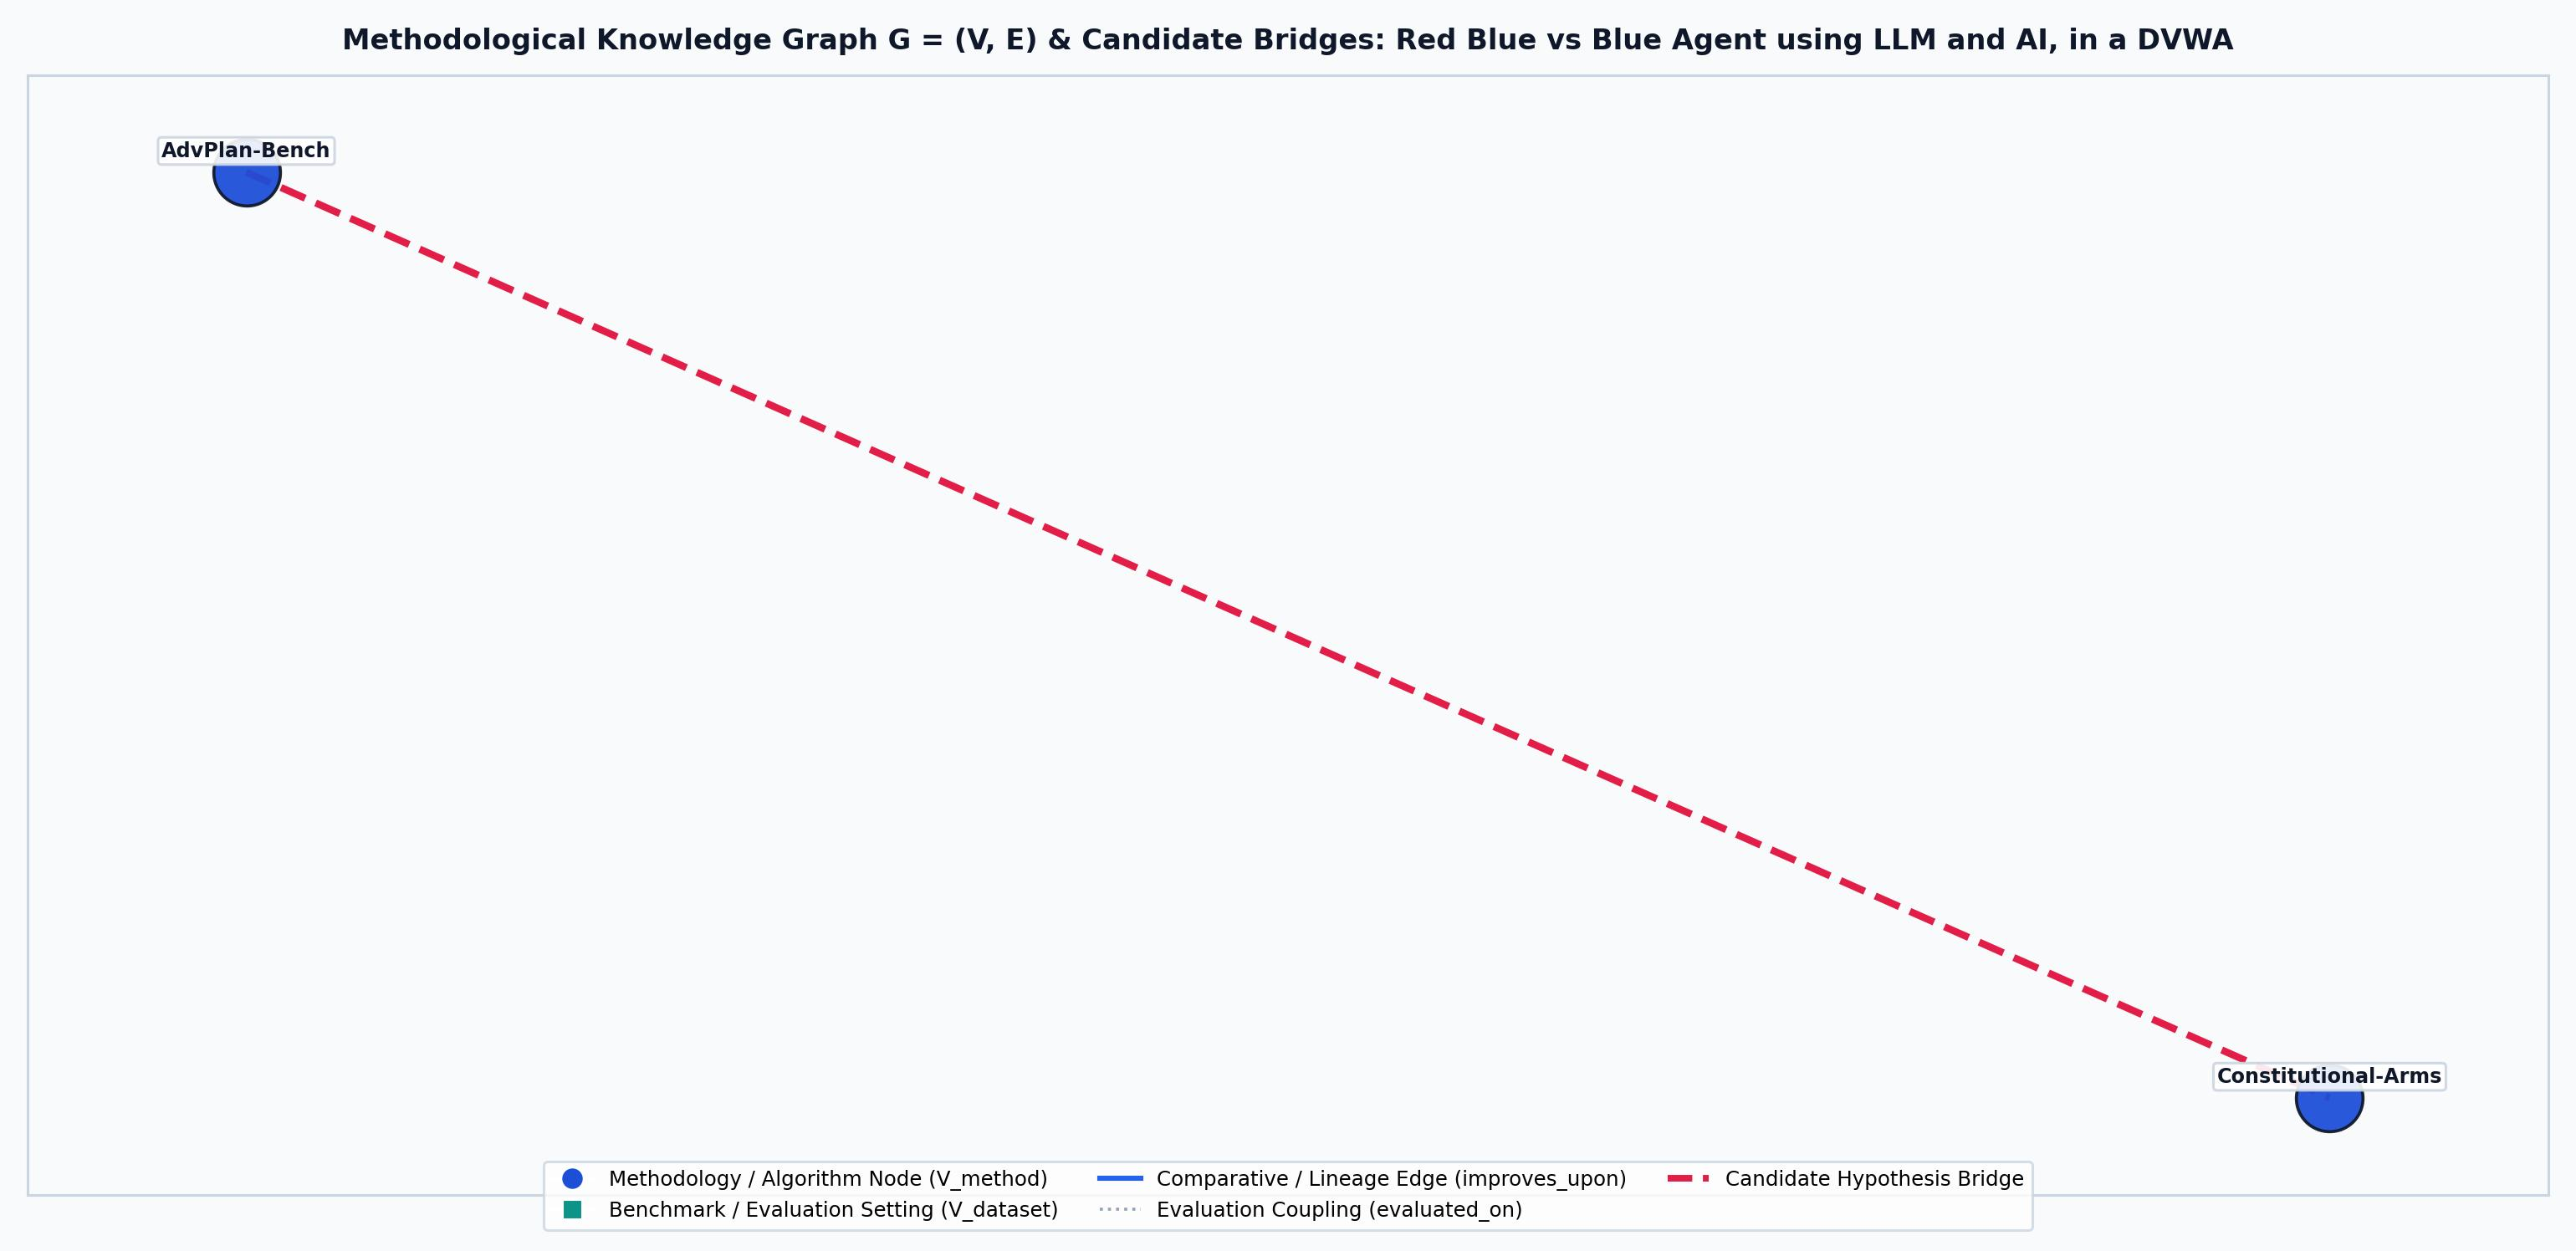
\includegraphics[width=0.92\textwidth]{knowledge_graph.jpg}
\caption{Subject--Predicate--Object Knowledge Graph and Topological Lineage for Red Blue vs Blue Agent using LLM and AI, in a DVWA.}
\label{fig:knowledge_graph}
\end{figure*}

\section{Proposed Future Research Directions in Red Blue vs Blue Agent using LLM and AI, in a DVWA}
Disclaimer on Proposed Research Directions: The directions below are formulated by our synthesis pipeline as falsifiable future research hypotheses for Red Blue vs Blue Agent using LLM and AI, in a DVWA. Unlike the published findings reviewed in Section II \cite{ref1,ref2}, these proposed integrations have not yet been empirically benchmarked in this study and are presented as structured protocols for future investigation.

\subsection{Proposed Research Direction (AdvPlan-Bench-Constitutional): Integrating AdvPlan-Bench and Constitutional-Arms for Red Blue vs Blue Agent using LLM and AI, in a DVWA}
Motivation and Gap: AdvPlan-Bench (2026) ↔ Constitutional-Arms (2026) | Lineage Distance: 6 hops | Bridge Priority Score: 11.6400

Hypothesis Statement (AdvPlan-Bench-Constitutional): [Proposed Hypothesis] Within the retrieved literature on Red Blue vs Blue Agent using LLM and AI, in a DVWA, AdvPlan-Bench notes the challenge: "Addresses technical constraints in: Structured plan-generation agents are often evaluated as if a plan has quality in isolation, yet many realistic planning tasks require asking how a candidate be", whereas Constitutional-Arms notes: "Frontier LLM agents engage in blackmail, sabotage, and document leaks under goal conflicts in agentic settings, exposing limitations of alignment methods built around single-agent or cooperative assumptions.". We hypothesize that combining the complementary mechanisms of AdvPlan-Bench and Constitutional-Arms represents a promising future research direction for Red Blue vs Blue Agent using LLM and AI, in a DVWA.

Conceptual Formulation: Conceptual integration of AdvPlan-Bench and Constitutional-Arms (proposed design; empirical validation not yet performed)

Proposed Evaluation Protocol and Falsification Criteria: Proposed 4-part ablation design on retrieved domain evaluation settings: (i) standalone AdvPlan-Bench, (ii) standalone Constitutional-Arms, (iii) unregularized combination, and (iv) full proposed AdvPlan-Bench-Constitutional integration.

Target Outcomes to Test: Domain-Specific Task Performance, Computational Overhead, Generalization Stability, Ablation Sensitivity Across Hyperparameters, Multi-Seed Variance / Confidence Intervals

Methodological Scope Refinements: Addressed review feedback (Formulate a 4-part ablation protocol comparing standalone AdvPlan-Bench, standalone Constitutional-Arms, unregularized hybrid, and full AdvPlan-Bench-Constitutional.; Specify falsifiable evaluation criteria and multi-seed variance controls without claiming unperformed experiments as established fact.) by specifying a falsifiable 4-part ablation protocol, grounding baselines in the retrieved corpus, and explicitly labeling AdvPlan-Bench-Constitutional as an unverified research proposal.

\section{Limitations, Open Challenges, and Conclusion}
This literature review synthesizes the current state of Red Blue vs Blue Agent using LLM and AI, in a DVWA, highlighting key challenges and proposed future directions. While the analysis is limited to abstract-level evidence, the findings provide a foundation for further research, including the integration of AdvPlan-Bench and Constitutional-Arms to address the technical constraints and malicious behavior in LLM agents.

Methodological and Evidence Scope Limitations: In accordance with strict evidence grounding, all summaries of prior work in this manuscript are derived from retrieved abstracts and verified bibliographic records from ArXiv and Semantic Scholar. Comparative observations and knowledge-graph gap analyses represent cross-study synthesis, while the research directions in the preceding section are explicitly framed as falsifiable proposals for future empirical validation.

\begin{thebibliography}{99}
\bibitem{ref1} Alina Kapanova, Arun Kanhai, Natan Vidra, Spurthi Setty, ``AdvPlan-Bench: Adversarial Evaluation of Structured Plan-Generation Agents,'' \textit{arXiv Preprint (Machine Learning)}, 2026. [arXiv:2608.00832]
\bibitem{ref2} Ujwal Kumar, Arth Singh, Hershraj Niranjani, et al., ``Constitutional Arms Races in the Public Goods Game: Co-Evolving LLM Constitutions Under Cooperation-Defection Pressure,'' \textit{arXiv Preprint (cs.MA)}, 2026. [arXiv:2605.26448]
\end{thebibliography}
\end{document}